\begin{figure}
  \setlength{\unitlength}{\textwidth}

        \begin{picture}(1,1.1)(0,0.35)

      % % % Parkinson Data 
      \put(0.1,1.1){\includegraphics[width=0.75\unitlength]{./chapter-cross-sections/fnp/vel_prof-tri-4.eps}}
      \put(0.1,0.737){\includegraphics[width=0.75\unitlength]{./chapter-cross-sections/fnp/vel_prof-tri-16.eps}}
      \put(0.1,0.38){\includegraphics[width=0.75\unitlength]{./chapter-cross-sections/fnp/vel_prof-tri-21.eps}}
     
      
      



%      
    \put(0.15,1.41){\small(a)}
     \put(0.15,1.05){\small(b)}
     \put(0.15,0.69){\small(c)}
\put(0.03,0.95){$\displaystyle\frac{V}{U}$}
\put(0.03,1.3){$\displaystyle\frac{A}{D}$}
\put(0.0,0.56){$\displaystyle\frac{P_{m}}{\rho \mathcal{A}U^3 }$}
\put(0.466,0.35){$\massdamp$}

      
    \end{picture}

    \caption{}
    \label{fig:surf_pres}
\end{figure}

 %vspace{10cm}
